% Created by tikzDevice version 0.12.6 on 2025-07-18 09:57:19
% !TEX encoding = UTF-8 Unicode
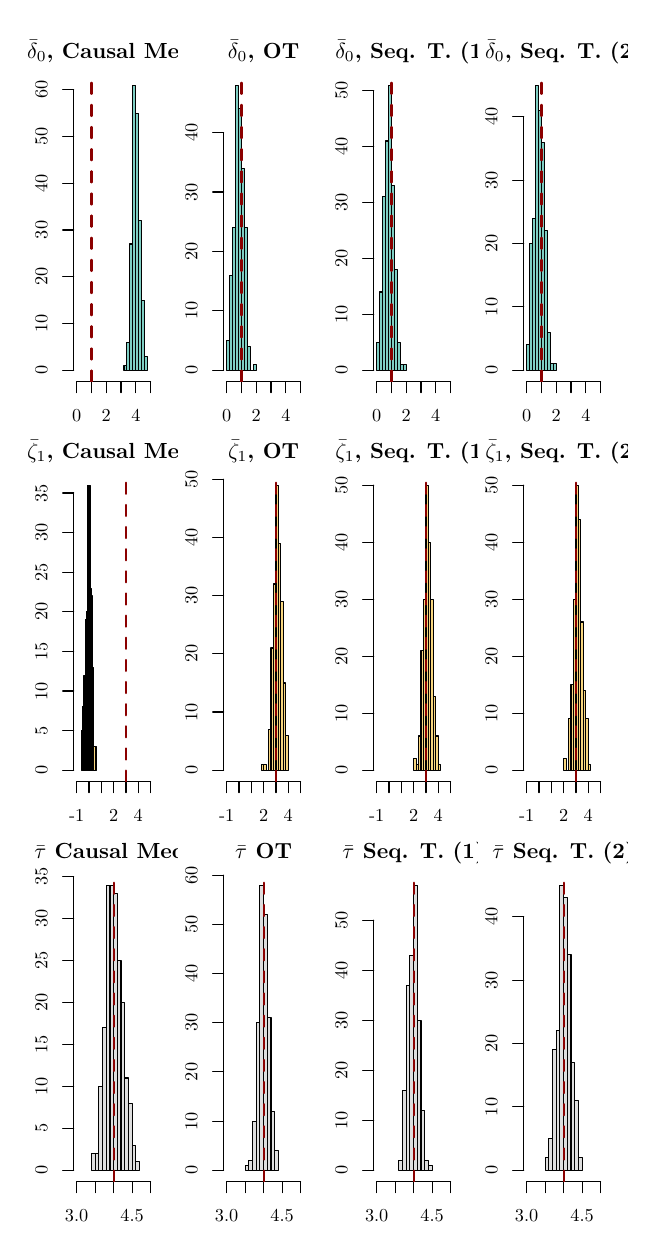
\begin{tikzpicture}[x=1pt,y=1pt]
\definecolor{fillColor}{RGB}{255,255,255}
\path[use as bounding box,fill=fillColor,fill opacity=0.00] (0,0) rectangle (216.81,433.62);
\begin{scope}
\path[clip] (  0.00,289.08) rectangle ( 54.20,433.62);
\definecolor{drawColor}{RGB}{0,0,0}

\node[text=drawColor,anchor=base,inner sep=0pt, outer sep=0pt, scale=  0.79] at ( 31.06,422.57) {\bfseries $\bar{\delta}_0$, Causal Med.};

\node[text=drawColor,rotate= 90.00,anchor=base,inner sep=0pt, outer sep=0pt, scale=  0.66] at ( -8.71,361.35) {Frequency};
\end{scope}
\begin{scope}
\path[clip] (  0.00,  0.00) rectangle (216.81,433.62);
\definecolor{drawColor}{RGB}{0,0,0}

\path[draw=drawColor,line width= 0.4pt,line join=round,line cap=round] ( 17.70,305.71) -- ( 44.42,305.71);

\path[draw=drawColor,line width= 0.4pt,line join=round,line cap=round] ( 17.70,305.71) -- ( 17.70,301.75);

\path[draw=drawColor,line width= 0.4pt,line join=round,line cap=round] ( 23.05,305.71) -- ( 23.05,301.75);

\path[draw=drawColor,line width= 0.4pt,line join=round,line cap=round] ( 28.39,305.71) -- ( 28.39,301.75);

\path[draw=drawColor,line width= 0.4pt,line join=round,line cap=round] ( 33.73,305.71) -- ( 33.73,301.75);

\path[draw=drawColor,line width= 0.4pt,line join=round,line cap=round] ( 39.08,305.71) -- ( 39.08,301.75);

\path[draw=drawColor,line width= 0.4pt,line join=round,line cap=round] ( 44.42,305.71) -- ( 44.42,301.75);

\node[text=drawColor,anchor=base,inner sep=0pt, outer sep=0pt, scale=  0.66] at ( 17.70,291.46) {0};

\node[text=drawColor,anchor=base,inner sep=0pt, outer sep=0pt, scale=  0.66] at ( 28.39,291.46) {2};

\node[text=drawColor,anchor=base,inner sep=0pt, outer sep=0pt, scale=  0.66] at ( 39.08,291.46) {4};

\path[draw=drawColor,line width= 0.4pt,line join=round,line cap=round] ( 16.63,309.83) -- ( 16.63,411.18);

\path[draw=drawColor,line width= 0.4pt,line join=round,line cap=round] ( 16.63,309.83) -- ( 12.67,309.83);

\path[draw=drawColor,line width= 0.4pt,line join=round,line cap=round] ( 16.63,326.72) -- ( 12.67,326.72);

\path[draw=drawColor,line width= 0.4pt,line join=round,line cap=round] ( 16.63,343.61) -- ( 12.67,343.61);

\path[draw=drawColor,line width= 0.4pt,line join=round,line cap=round] ( 16.63,360.51) -- ( 12.67,360.51);

\path[draw=drawColor,line width= 0.4pt,line join=round,line cap=round] ( 16.63,377.40) -- ( 12.67,377.40);

\path[draw=drawColor,line width= 0.4pt,line join=round,line cap=round] ( 16.63,394.29) -- ( 12.67,394.29);

\path[draw=drawColor,line width= 0.4pt,line join=round,line cap=round] ( 16.63,411.18) -- ( 12.67,411.18);

\node[text=drawColor,rotate= 90.00,anchor=base,inner sep=0pt, outer sep=0pt, scale=  0.66] at (  7.13,309.83) {0};

\node[text=drawColor,rotate= 90.00,anchor=base,inner sep=0pt, outer sep=0pt, scale=  0.66] at (  7.13,326.72) {10};

\node[text=drawColor,rotate= 90.00,anchor=base,inner sep=0pt, outer sep=0pt, scale=  0.66] at (  7.13,343.61) {20};

\node[text=drawColor,rotate= 90.00,anchor=base,inner sep=0pt, outer sep=0pt, scale=  0.66] at (  7.13,360.51) {30};

\node[text=drawColor,rotate= 90.00,anchor=base,inner sep=0pt, outer sep=0pt, scale=  0.66] at (  7.13,377.40) {40};

\node[text=drawColor,rotate= 90.00,anchor=base,inner sep=0pt, outer sep=0pt, scale=  0.66] at (  7.13,394.29) {50};

\node[text=drawColor,rotate= 90.00,anchor=base,inner sep=0pt, outer sep=0pt, scale=  0.66] at (  7.13,411.18) {60};
\end{scope}
\begin{scope}
\path[clip] ( 16.63,305.71) rectangle ( 45.49,416.99);
\definecolor{drawColor}{RGB}{0,0,0}
\definecolor{fillColor}{RGB}{0,160,138}

\path[draw=drawColor,line width= 0.4pt,line join=round,line cap=round,fill=fillColor,fill opacity=0.50] ( 34.80,309.83) rectangle ( 35.87,311.52);

\path[draw=drawColor,line width= 0.4pt,line join=round,line cap=round,fill=fillColor,fill opacity=0.50] ( 35.87,309.83) rectangle ( 36.94,319.97);

\path[draw=drawColor,line width= 0.4pt,line join=round,line cap=round,fill=fillColor,fill opacity=0.50] ( 36.94,309.83) rectangle ( 38.01,355.44);

\path[draw=drawColor,line width= 0.4pt,line join=round,line cap=round,fill=fillColor,fill opacity=0.50] ( 38.01,309.83) rectangle ( 39.08,412.87);

\path[draw=drawColor,line width= 0.4pt,line join=round,line cap=round,fill=fillColor,fill opacity=0.50] ( 39.08,309.83) rectangle ( 40.15,402.73);

\path[draw=drawColor,line width= 0.4pt,line join=round,line cap=round,fill=fillColor,fill opacity=0.50] ( 40.15,309.83) rectangle ( 41.22,363.88);

\path[draw=drawColor,line width= 0.4pt,line join=round,line cap=round,fill=fillColor,fill opacity=0.50] ( 41.22,309.83) rectangle ( 42.28,335.17);

\path[draw=drawColor,line width= 0.4pt,line join=round,line cap=round,fill=fillColor,fill opacity=0.50] ( 42.28,309.83) rectangle ( 43.35,314.90);
\definecolor{drawColor}{RGB}{139,0,0}

\path[draw=drawColor,line width= 0.8pt,dash pattern=on 4pt off 4pt ,line join=round,line cap=round] ( 23.05,305.71) -- ( 23.05,416.99);
\end{scope}
\begin{scope}
\path[clip] ( 54.20,289.08) rectangle (108.41,433.62);
\definecolor{drawColor}{RGB}{0,0,0}

\node[text=drawColor,anchor=base,inner sep=0pt, outer sep=0pt, scale=  0.79] at ( 85.26,422.57) {\bfseries $\bar{\delta}_0$, OT};

\node[text=drawColor,rotate= 90.00,anchor=base,inner sep=0pt, outer sep=0pt, scale=  0.66] at ( 45.49,361.35) {Frequency};
\end{scope}
\begin{scope}
\path[clip] (  0.00,  0.00) rectangle (216.81,433.62);
\definecolor{drawColor}{RGB}{0,0,0}

\path[draw=drawColor,line width= 0.4pt,line join=round,line cap=round] ( 71.90,305.71) -- ( 98.62,305.71);

\path[draw=drawColor,line width= 0.4pt,line join=round,line cap=round] ( 71.90,305.71) -- ( 71.90,301.75);

\path[draw=drawColor,line width= 0.4pt,line join=round,line cap=round] ( 77.25,305.71) -- ( 77.25,301.75);

\path[draw=drawColor,line width= 0.4pt,line join=round,line cap=round] ( 82.59,305.71) -- ( 82.59,301.75);

\path[draw=drawColor,line width= 0.4pt,line join=round,line cap=round] ( 87.94,305.71) -- ( 87.94,301.75);

\path[draw=drawColor,line width= 0.4pt,line join=round,line cap=round] ( 93.28,305.71) -- ( 93.28,301.75);

\path[draw=drawColor,line width= 0.4pt,line join=round,line cap=round] ( 98.62,305.71) -- ( 98.62,301.75);

\node[text=drawColor,anchor=base,inner sep=0pt, outer sep=0pt, scale=  0.66] at ( 71.90,291.46) {0};

\node[text=drawColor,anchor=base,inner sep=0pt, outer sep=0pt, scale=  0.66] at ( 82.59,291.46) {2};

\node[text=drawColor,anchor=base,inner sep=0pt, outer sep=0pt, scale=  0.66] at ( 93.28,291.46) {4};

\path[draw=drawColor,line width= 0.4pt,line join=round,line cap=round] ( 70.83,309.83) -- ( 70.83,395.69);

\path[draw=drawColor,line width= 0.4pt,line join=round,line cap=round] ( 70.83,309.83) -- ( 66.87,309.83);

\path[draw=drawColor,line width= 0.4pt,line join=round,line cap=round] ( 70.83,331.30) -- ( 66.87,331.30);

\path[draw=drawColor,line width= 0.4pt,line join=round,line cap=round] ( 70.83,352.76) -- ( 66.87,352.76);

\path[draw=drawColor,line width= 0.4pt,line join=round,line cap=round] ( 70.83,374.23) -- ( 66.87,374.23);

\path[draw=drawColor,line width= 0.4pt,line join=round,line cap=round] ( 70.83,395.69) -- ( 66.87,395.69);

\node[text=drawColor,rotate= 90.00,anchor=base,inner sep=0pt, outer sep=0pt, scale=  0.66] at ( 61.33,309.83) {0};

\node[text=drawColor,rotate= 90.00,anchor=base,inner sep=0pt, outer sep=0pt, scale=  0.66] at ( 61.33,331.30) {10};

\node[text=drawColor,rotate= 90.00,anchor=base,inner sep=0pt, outer sep=0pt, scale=  0.66] at ( 61.33,352.76) {20};

\node[text=drawColor,rotate= 90.00,anchor=base,inner sep=0pt, outer sep=0pt, scale=  0.66] at ( 61.33,374.23) {30};

\node[text=drawColor,rotate= 90.00,anchor=base,inner sep=0pt, outer sep=0pt, scale=  0.66] at ( 61.33,395.69) {40};
\end{scope}
\begin{scope}
\path[clip] ( 70.83,305.71) rectangle ( 99.69,416.99);
\definecolor{drawColor}{RGB}{0,0,0}
\definecolor{fillColor}{RGB}{0,160,138}

\path[draw=drawColor,line width= 0.4pt,line join=round,line cap=round,fill=fillColor,fill opacity=0.50] ( 71.90,309.83) rectangle ( 72.97,320.57);

\path[draw=drawColor,line width= 0.4pt,line join=round,line cap=round,fill=fillColor,fill opacity=0.50] ( 72.97,309.83) rectangle ( 74.04,344.18);

\path[draw=drawColor,line width= 0.4pt,line join=round,line cap=round,fill=fillColor,fill opacity=0.50] ( 74.04,309.83) rectangle ( 75.11,361.35);

\path[draw=drawColor,line width= 0.4pt,line join=round,line cap=round,fill=fillColor,fill opacity=0.50] ( 75.11,309.83) rectangle ( 76.18,412.87);

\path[draw=drawColor,line width= 0.4pt,line join=round,line cap=round,fill=fillColor,fill opacity=0.50] ( 76.18,309.83) rectangle ( 77.25,404.28);

\path[draw=drawColor,line width= 0.4pt,line join=round,line cap=round,fill=fillColor,fill opacity=0.50] ( 77.25,309.83) rectangle ( 78.32,382.82);

\path[draw=drawColor,line width= 0.4pt,line join=round,line cap=round,fill=fillColor,fill opacity=0.50] ( 78.32,309.83) rectangle ( 79.39,361.35);

\path[draw=drawColor,line width= 0.4pt,line join=round,line cap=round,fill=fillColor,fill opacity=0.50] ( 79.39,309.83) rectangle ( 80.45,318.42);

\path[draw=drawColor,line width= 0.4pt,line join=round,line cap=round,fill=fillColor,fill opacity=0.50] ( 80.45,309.83) rectangle ( 81.52,309.83);

\path[draw=drawColor,line width= 0.4pt,line join=round,line cap=round,fill=fillColor,fill opacity=0.50] ( 81.52,309.83) rectangle ( 82.59,311.98);
\definecolor{drawColor}{RGB}{139,0,0}

\path[draw=drawColor,line width= 0.8pt,dash pattern=on 4pt off 4pt ,line join=round,line cap=round] ( 77.25,305.71) -- ( 77.25,416.99);
\end{scope}
\begin{scope}
\path[clip] (108.41,289.08) rectangle (162.61,433.62);
\definecolor{drawColor}{RGB}{0,0,0}

\node[text=drawColor,anchor=base,inner sep=0pt, outer sep=0pt, scale=  0.79] at (139.47,422.57) {\bfseries $\bar{\delta}_0$, Seq. T. (1)};

\node[text=drawColor,rotate= 90.00,anchor=base,inner sep=0pt, outer sep=0pt, scale=  0.66] at ( 99.69,361.35) {Frequency};
\end{scope}
\begin{scope}
\path[clip] (  0.00,  0.00) rectangle (216.81,433.62);
\definecolor{drawColor}{RGB}{0,0,0}

\path[draw=drawColor,line width= 0.4pt,line join=round,line cap=round] (126.11,305.71) -- (152.83,305.71);

\path[draw=drawColor,line width= 0.4pt,line join=round,line cap=round] (126.11,305.71) -- (126.11,301.75);

\path[draw=drawColor,line width= 0.4pt,line join=round,line cap=round] (131.45,305.71) -- (131.45,301.75);

\path[draw=drawColor,line width= 0.4pt,line join=round,line cap=round] (136.79,305.71) -- (136.79,301.75);

\path[draw=drawColor,line width= 0.4pt,line join=round,line cap=round] (142.14,305.71) -- (142.14,301.75);

\path[draw=drawColor,line width= 0.4pt,line join=round,line cap=round] (147.48,305.71) -- (147.48,301.75);

\path[draw=drawColor,line width= 0.4pt,line join=round,line cap=round] (152.83,305.71) -- (152.83,301.75);

\node[text=drawColor,anchor=base,inner sep=0pt, outer sep=0pt, scale=  0.66] at (126.11,291.46) {0};

\node[text=drawColor,anchor=base,inner sep=0pt, outer sep=0pt, scale=  0.66] at (136.79,291.46) {2};

\node[text=drawColor,anchor=base,inner sep=0pt, outer sep=0pt, scale=  0.66] at (147.48,291.46) {4};

\path[draw=drawColor,line width= 0.4pt,line join=round,line cap=round] (125.04,309.83) -- (125.04,410.85);

\path[draw=drawColor,line width= 0.4pt,line join=round,line cap=round] (125.04,309.83) -- (121.08,309.83);

\path[draw=drawColor,line width= 0.4pt,line join=round,line cap=round] (125.04,330.04) -- (121.08,330.04);

\path[draw=drawColor,line width= 0.4pt,line join=round,line cap=round] (125.04,350.24) -- (121.08,350.24);

\path[draw=drawColor,line width= 0.4pt,line join=round,line cap=round] (125.04,370.44) -- (121.08,370.44);

\path[draw=drawColor,line width= 0.4pt,line join=round,line cap=round] (125.04,390.64) -- (121.08,390.64);

\path[draw=drawColor,line width= 0.4pt,line join=round,line cap=round] (125.04,410.85) -- (121.08,410.85);

\node[text=drawColor,rotate= 90.00,anchor=base,inner sep=0pt, outer sep=0pt, scale=  0.66] at (115.53,309.83) {0};

\node[text=drawColor,rotate= 90.00,anchor=base,inner sep=0pt, outer sep=0pt, scale=  0.66] at (115.53,330.04) {10};

\node[text=drawColor,rotate= 90.00,anchor=base,inner sep=0pt, outer sep=0pt, scale=  0.66] at (115.53,350.24) {20};

\node[text=drawColor,rotate= 90.00,anchor=base,inner sep=0pt, outer sep=0pt, scale=  0.66] at (115.53,370.44) {30};

\node[text=drawColor,rotate= 90.00,anchor=base,inner sep=0pt, outer sep=0pt, scale=  0.66] at (115.53,390.64) {40};

\node[text=drawColor,rotate= 90.00,anchor=base,inner sep=0pt, outer sep=0pt, scale=  0.66] at (115.53,410.85) {50};
\end{scope}
\begin{scope}
\path[clip] (125.04,305.71) rectangle (153.90,416.99);
\definecolor{drawColor}{RGB}{0,0,0}
\definecolor{fillColor}{RGB}{0,160,138}

\path[draw=drawColor,line width= 0.4pt,line join=round,line cap=round,fill=fillColor,fill opacity=0.50] (126.11,309.83) rectangle (127.17,319.93);

\path[draw=drawColor,line width= 0.4pt,line join=round,line cap=round,fill=fillColor,fill opacity=0.50] (127.17,309.83) rectangle (128.24,338.12);

\path[draw=drawColor,line width= 0.4pt,line join=round,line cap=round,fill=fillColor,fill opacity=0.50] (128.24,309.83) rectangle (129.31,372.46);

\path[draw=drawColor,line width= 0.4pt,line join=round,line cap=round,fill=fillColor,fill opacity=0.50] (129.31,309.83) rectangle (130.38,392.66);

\path[draw=drawColor,line width= 0.4pt,line join=round,line cap=round,fill=fillColor,fill opacity=0.50] (130.38,309.83) rectangle (131.45,412.87);

\path[draw=drawColor,line width= 0.4pt,line join=round,line cap=round,fill=fillColor,fill opacity=0.50] (131.45,309.83) rectangle (132.52,376.50);

\path[draw=drawColor,line width= 0.4pt,line join=round,line cap=round,fill=fillColor,fill opacity=0.50] (132.52,309.83) rectangle (133.59,346.20);

\path[draw=drawColor,line width= 0.4pt,line join=round,line cap=round,fill=fillColor,fill opacity=0.50] (133.59,309.83) rectangle (134.66,319.93);

\path[draw=drawColor,line width= 0.4pt,line join=round,line cap=round,fill=fillColor,fill opacity=0.50] (134.66,309.83) rectangle (135.73,311.85);

\path[draw=drawColor,line width= 0.4pt,line join=round,line cap=round,fill=fillColor,fill opacity=0.50] (135.73,309.83) rectangle (136.79,311.85);
\definecolor{drawColor}{RGB}{139,0,0}

\path[draw=drawColor,line width= 0.8pt,dash pattern=on 4pt off 4pt ,line join=round,line cap=round] (131.45,305.71) -- (131.45,416.99);
\end{scope}
\begin{scope}
\path[clip] (162.61,289.08) rectangle (216.81,433.62);
\definecolor{drawColor}{RGB}{0,0,0}

\node[text=drawColor,anchor=base,inner sep=0pt, outer sep=0pt, scale=  0.79] at (193.67,422.57) {\bfseries $\bar{\delta}_0$, Seq. T. (2)};

\node[text=drawColor,rotate= 90.00,anchor=base,inner sep=0pt, outer sep=0pt, scale=  0.66] at (153.90,361.35) {Frequency};
\end{scope}
\begin{scope}
\path[clip] (  0.00,  0.00) rectangle (216.81,433.62);
\definecolor{drawColor}{RGB}{0,0,0}

\path[draw=drawColor,line width= 0.4pt,line join=round,line cap=round] (180.31,305.71) -- (207.03,305.71);

\path[draw=drawColor,line width= 0.4pt,line join=round,line cap=round] (180.31,305.71) -- (180.31,301.75);

\path[draw=drawColor,line width= 0.4pt,line join=round,line cap=round] (185.65,305.71) -- (185.65,301.75);

\path[draw=drawColor,line width= 0.4pt,line join=round,line cap=round] (191.00,305.71) -- (191.00,301.75);

\path[draw=drawColor,line width= 0.4pt,line join=round,line cap=round] (196.34,305.71) -- (196.34,301.75);

\path[draw=drawColor,line width= 0.4pt,line join=round,line cap=round] (201.69,305.71) -- (201.69,301.75);

\path[draw=drawColor,line width= 0.4pt,line join=round,line cap=round] (207.03,305.71) -- (207.03,301.75);

\node[text=drawColor,anchor=base,inner sep=0pt, outer sep=0pt, scale=  0.66] at (180.31,291.46) {0};

\node[text=drawColor,anchor=base,inner sep=0pt, outer sep=0pt, scale=  0.66] at (191.00,291.46) {2};

\node[text=drawColor,anchor=base,inner sep=0pt, outer sep=0pt, scale=  0.66] at (201.69,291.46) {4};

\path[draw=drawColor,line width= 0.4pt,line join=round,line cap=round] (179.24,309.83) -- (179.24,401.42);

\path[draw=drawColor,line width= 0.4pt,line join=round,line cap=round] (179.24,309.83) -- (175.28,309.83);

\path[draw=drawColor,line width= 0.4pt,line join=round,line cap=round] (179.24,332.73) -- (175.28,332.73);

\path[draw=drawColor,line width= 0.4pt,line join=round,line cap=round] (179.24,355.63) -- (175.28,355.63);

\path[draw=drawColor,line width= 0.4pt,line join=round,line cap=round] (179.24,378.52) -- (175.28,378.52);

\path[draw=drawColor,line width= 0.4pt,line join=round,line cap=round] (179.24,401.42) -- (175.28,401.42);

\node[text=drawColor,rotate= 90.00,anchor=base,inner sep=0pt, outer sep=0pt, scale=  0.66] at (169.74,309.83) {0};

\node[text=drawColor,rotate= 90.00,anchor=base,inner sep=0pt, outer sep=0pt, scale=  0.66] at (169.74,332.73) {10};

\node[text=drawColor,rotate= 90.00,anchor=base,inner sep=0pt, outer sep=0pt, scale=  0.66] at (169.74,355.63) {20};

\node[text=drawColor,rotate= 90.00,anchor=base,inner sep=0pt, outer sep=0pt, scale=  0.66] at (169.74,378.52) {30};

\node[text=drawColor,rotate= 90.00,anchor=base,inner sep=0pt, outer sep=0pt, scale=  0.66] at (169.74,401.42) {40};
\end{scope}
\begin{scope}
\path[clip] (179.24,305.71) rectangle (208.10,416.99);
\definecolor{drawColor}{RGB}{0,0,0}
\definecolor{fillColor}{RGB}{0,160,138}

\path[draw=drawColor,line width= 0.4pt,line join=round,line cap=round,fill=fillColor,fill opacity=0.50] (180.31,309.83) rectangle (181.38,318.99);

\path[draw=drawColor,line width= 0.4pt,line join=round,line cap=round,fill=fillColor,fill opacity=0.50] (181.38,309.83) rectangle (182.45,355.63);

\path[draw=drawColor,line width= 0.4pt,line join=round,line cap=round,fill=fillColor,fill opacity=0.50] (182.45,309.83) rectangle (183.51,364.78);

\path[draw=drawColor,line width= 0.4pt,line join=round,line cap=round,fill=fillColor,fill opacity=0.50] (183.51,309.83) rectangle (184.58,412.87);

\path[draw=drawColor,line width= 0.4pt,line join=round,line cap=round,fill=fillColor,fill opacity=0.50] (184.58,309.83) rectangle (185.65,403.71);

\path[draw=drawColor,line width= 0.4pt,line join=round,line cap=round,fill=fillColor,fill opacity=0.50] (185.65,309.83) rectangle (186.72,392.26);

\path[draw=drawColor,line width= 0.4pt,line join=round,line cap=round,fill=fillColor,fill opacity=0.50] (186.72,309.83) rectangle (187.79,360.21);

\path[draw=drawColor,line width= 0.4pt,line join=round,line cap=round,fill=fillColor,fill opacity=0.50] (187.79,309.83) rectangle (188.86,323.57);

\path[draw=drawColor,line width= 0.4pt,line join=round,line cap=round,fill=fillColor,fill opacity=0.50] (188.86,309.83) rectangle (189.93,312.12);

\path[draw=drawColor,line width= 0.4pt,line join=round,line cap=round,fill=fillColor,fill opacity=0.50] (189.93,309.83) rectangle (191.00,312.12);
\definecolor{drawColor}{RGB}{139,0,0}

\path[draw=drawColor,line width= 0.8pt,dash pattern=on 4pt off 4pt ,line join=round,line cap=round] (185.65,305.71) -- (185.65,416.99);
\end{scope}
\begin{scope}
\path[clip] (  0.00,144.54) rectangle ( 54.20,289.08);
\definecolor{drawColor}{RGB}{0,0,0}

\node[text=drawColor,anchor=base,inner sep=0pt, outer sep=0pt, scale=  0.79] at ( 31.06,278.03) {\bfseries $\bar{\zeta}_1$, Causal Med.};

\node[text=drawColor,rotate= 90.00,anchor=base,inner sep=0pt, outer sep=0pt, scale=  0.66] at ( -8.71,216.81) {Frequency};
\end{scope}
\begin{scope}
\path[clip] (  0.00,  0.00) rectangle (216.81,433.62);
\definecolor{drawColor}{RGB}{0,0,0}

\path[draw=drawColor,line width= 0.4pt,line join=round,line cap=round] ( 17.70,161.17) -- ( 44.42,161.17);

\path[draw=drawColor,line width= 0.4pt,line join=round,line cap=round] ( 17.70,161.17) -- ( 17.70,157.21);

\path[draw=drawColor,line width= 0.4pt,line join=round,line cap=round] ( 22.15,161.17) -- ( 22.15,157.21);

\path[draw=drawColor,line width= 0.4pt,line join=round,line cap=round] ( 26.61,161.17) -- ( 26.61,157.21);

\path[draw=drawColor,line width= 0.4pt,line join=round,line cap=round] ( 31.06,161.17) -- ( 31.06,157.21);

\path[draw=drawColor,line width= 0.4pt,line join=round,line cap=round] ( 35.51,161.17) -- ( 35.51,157.21);

\path[draw=drawColor,line width= 0.4pt,line join=round,line cap=round] ( 39.97,161.17) -- ( 39.97,157.21);

\path[draw=drawColor,line width= 0.4pt,line join=round,line cap=round] ( 44.42,161.17) -- ( 44.42,157.21);

\node[text=drawColor,anchor=base,inner sep=0pt, outer sep=0pt, scale=  0.66] at ( 17.70,146.92) {-1};

\node[text=drawColor,anchor=base,inner sep=0pt, outer sep=0pt, scale=  0.66] at ( 31.06,146.92) {2};

\node[text=drawColor,anchor=base,inner sep=0pt, outer sep=0pt, scale=  0.66] at ( 39.97,146.92) {4};

\path[draw=drawColor,line width= 0.4pt,line join=round,line cap=round] ( 16.63,165.29) -- ( 16.63,265.46);

\path[draw=drawColor,line width= 0.4pt,line join=round,line cap=round] ( 16.63,165.29) -- ( 12.67,165.29);

\path[draw=drawColor,line width= 0.4pt,line join=round,line cap=round] ( 16.63,179.60) -- ( 12.67,179.60);

\path[draw=drawColor,line width= 0.4pt,line join=round,line cap=round] ( 16.63,193.91) -- ( 12.67,193.91);

\path[draw=drawColor,line width= 0.4pt,line join=round,line cap=round] ( 16.63,208.22) -- ( 12.67,208.22);

\path[draw=drawColor,line width= 0.4pt,line join=round,line cap=round] ( 16.63,222.53) -- ( 12.67,222.53);

\path[draw=drawColor,line width= 0.4pt,line join=round,line cap=round] ( 16.63,236.84) -- ( 12.67,236.84);

\path[draw=drawColor,line width= 0.4pt,line join=round,line cap=round] ( 16.63,251.15) -- ( 12.67,251.15);

\path[draw=drawColor,line width= 0.4pt,line join=round,line cap=round] ( 16.63,265.46) -- ( 12.67,265.46);

\node[text=drawColor,rotate= 90.00,anchor=base,inner sep=0pt, outer sep=0pt, scale=  0.66] at (  7.13,165.29) {0};

\node[text=drawColor,rotate= 90.00,anchor=base,inner sep=0pt, outer sep=0pt, scale=  0.66] at (  7.13,179.60) {5};

\node[text=drawColor,rotate= 90.00,anchor=base,inner sep=0pt, outer sep=0pt, scale=  0.66] at (  7.13,193.91) {10};

\node[text=drawColor,rotate= 90.00,anchor=base,inner sep=0pt, outer sep=0pt, scale=  0.66] at (  7.13,208.22) {15};

\node[text=drawColor,rotate= 90.00,anchor=base,inner sep=0pt, outer sep=0pt, scale=  0.66] at (  7.13,222.53) {20};

\node[text=drawColor,rotate= 90.00,anchor=base,inner sep=0pt, outer sep=0pt, scale=  0.66] at (  7.13,236.84) {25};

\node[text=drawColor,rotate= 90.00,anchor=base,inner sep=0pt, outer sep=0pt, scale=  0.66] at (  7.13,251.15) {30};

\node[text=drawColor,rotate= 90.00,anchor=base,inner sep=0pt, outer sep=0pt, scale=  0.66] at (  7.13,265.46) {35};
\end{scope}
\begin{scope}
\path[clip] ( 16.63,161.17) rectangle ( 45.49,272.45);
\definecolor{drawColor}{RGB}{0,0,0}
\definecolor{fillColor}{RGB}{242,173,0}

\path[draw=drawColor,line width= 0.4pt,line join=round,line cap=round,fill=fillColor,fill opacity=0.50] ( 19.48,165.29) rectangle ( 19.93,179.60);

\path[draw=drawColor,line width= 0.4pt,line join=round,line cap=round,fill=fillColor,fill opacity=0.50] ( 19.93,165.29) rectangle ( 20.37,188.19);

\path[draw=drawColor,line width= 0.4pt,line join=round,line cap=round,fill=fillColor,fill opacity=0.50] ( 20.37,165.29) rectangle ( 20.82,199.64);

\path[draw=drawColor,line width= 0.4pt,line join=round,line cap=round,fill=fillColor,fill opacity=0.50] ( 20.82,165.29) rectangle ( 21.26,219.67);

\path[draw=drawColor,line width= 0.4pt,line join=round,line cap=round,fill=fillColor,fill opacity=0.50] ( 21.26,165.29) rectangle ( 21.71,222.53);

\path[draw=drawColor,line width= 0.4pt,line join=round,line cap=round,fill=fillColor,fill opacity=0.50] ( 21.71,165.29) rectangle ( 22.15,268.33);

\path[draw=drawColor,line width= 0.4pt,line join=round,line cap=round,fill=fillColor,fill opacity=0.50] ( 22.15,165.29) rectangle ( 22.60,268.33);

\path[draw=drawColor,line width= 0.4pt,line join=round,line cap=round,fill=fillColor,fill opacity=0.50] ( 22.60,165.29) rectangle ( 23.05,231.12);

\path[draw=drawColor,line width= 0.4pt,line join=round,line cap=round,fill=fillColor,fill opacity=0.50] ( 23.05,165.29) rectangle ( 23.49,228.26);

\path[draw=drawColor,line width= 0.4pt,line join=round,line cap=round,fill=fillColor,fill opacity=0.50] ( 23.49,165.29) rectangle ( 23.94,202.50);

\path[draw=drawColor,line width= 0.4pt,line join=round,line cap=round,fill=fillColor,fill opacity=0.50] ( 23.94,165.29) rectangle ( 24.38,173.88);

\path[draw=drawColor,line width= 0.4pt,line join=round,line cap=round,fill=fillColor,fill opacity=0.50] ( 24.38,165.29) rectangle ( 24.83,173.88);
\definecolor{drawColor}{RGB}{139,0,0}

\path[draw=drawColor,line width= 0.8pt,dash pattern=on 4pt off 4pt ,line join=round,line cap=round] ( 35.51,161.17) -- ( 35.51,272.45);
\end{scope}
\begin{scope}
\path[clip] ( 54.20,144.54) rectangle (108.41,289.08);
\definecolor{drawColor}{RGB}{0,0,0}

\node[text=drawColor,anchor=base,inner sep=0pt, outer sep=0pt, scale=  0.79] at ( 85.26,278.03) {\bfseries $\bar{\zeta}_1$, OT};

\node[text=drawColor,rotate= 90.00,anchor=base,inner sep=0pt, outer sep=0pt, scale=  0.66] at ( 45.49,216.81) {Frequency};
\end{scope}
\begin{scope}
\path[clip] (  0.00,  0.00) rectangle (216.81,433.62);
\definecolor{drawColor}{RGB}{0,0,0}

\path[draw=drawColor,line width= 0.4pt,line join=round,line cap=round] ( 71.90,161.17) -- ( 98.62,161.17);

\path[draw=drawColor,line width= 0.4pt,line join=round,line cap=round] ( 71.90,161.17) -- ( 71.90,157.21);

\path[draw=drawColor,line width= 0.4pt,line join=round,line cap=round] ( 76.36,161.17) -- ( 76.36,157.21);

\path[draw=drawColor,line width= 0.4pt,line join=round,line cap=round] ( 80.81,161.17) -- ( 80.81,157.21);

\path[draw=drawColor,line width= 0.4pt,line join=round,line cap=round] ( 85.26,161.17) -- ( 85.26,157.21);

\path[draw=drawColor,line width= 0.4pt,line join=round,line cap=round] ( 89.72,161.17) -- ( 89.72,157.21);

\path[draw=drawColor,line width= 0.4pt,line join=round,line cap=round] ( 94.17,161.17) -- ( 94.17,157.21);

\path[draw=drawColor,line width= 0.4pt,line join=round,line cap=round] ( 98.62,161.17) -- ( 98.62,157.21);

\node[text=drawColor,anchor=base,inner sep=0pt, outer sep=0pt, scale=  0.66] at ( 71.90,146.92) {-1};

\node[text=drawColor,anchor=base,inner sep=0pt, outer sep=0pt, scale=  0.66] at ( 85.26,146.92) {2};

\node[text=drawColor,anchor=base,inner sep=0pt, outer sep=0pt, scale=  0.66] at ( 94.17,146.92) {4};

\path[draw=drawColor,line width= 0.4pt,line join=round,line cap=round] ( 70.83,165.29) -- ( 70.83,270.43);

\path[draw=drawColor,line width= 0.4pt,line join=round,line cap=round] ( 70.83,165.29) -- ( 66.87,165.29);

\path[draw=drawColor,line width= 0.4pt,line join=round,line cap=round] ( 70.83,186.32) -- ( 66.87,186.32);

\path[draw=drawColor,line width= 0.4pt,line join=round,line cap=round] ( 70.83,207.35) -- ( 66.87,207.35);

\path[draw=drawColor,line width= 0.4pt,line join=round,line cap=round] ( 70.83,228.37) -- ( 66.87,228.37);

\path[draw=drawColor,line width= 0.4pt,line join=round,line cap=round] ( 70.83,249.40) -- ( 66.87,249.40);

\path[draw=drawColor,line width= 0.4pt,line join=round,line cap=round] ( 70.83,270.43) -- ( 66.87,270.43);

\node[text=drawColor,rotate= 90.00,anchor=base,inner sep=0pt, outer sep=0pt, scale=  0.66] at ( 61.33,165.29) {0};

\node[text=drawColor,rotate= 90.00,anchor=base,inner sep=0pt, outer sep=0pt, scale=  0.66] at ( 61.33,186.32) {10};

\node[text=drawColor,rotate= 90.00,anchor=base,inner sep=0pt, outer sep=0pt, scale=  0.66] at ( 61.33,207.35) {20};

\node[text=drawColor,rotate= 90.00,anchor=base,inner sep=0pt, outer sep=0pt, scale=  0.66] at ( 61.33,228.37) {30};

\node[text=drawColor,rotate= 90.00,anchor=base,inner sep=0pt, outer sep=0pt, scale=  0.66] at ( 61.33,249.40) {40};

\node[text=drawColor,rotate= 90.00,anchor=base,inner sep=0pt, outer sep=0pt, scale=  0.66] at ( 61.33,270.43) {50};
\end{scope}
\begin{scope}
\path[clip] ( 70.83,161.17) rectangle ( 99.69,272.45);
\definecolor{drawColor}{RGB}{0,0,0}
\definecolor{fillColor}{RGB}{242,173,0}

\path[draw=drawColor,line width= 0.4pt,line join=round,line cap=round,fill=fillColor,fill opacity=0.50] ( 84.37,165.29) rectangle ( 85.26,167.40);

\path[draw=drawColor,line width= 0.4pt,line join=round,line cap=round,fill=fillColor,fill opacity=0.50] ( 85.26,165.29) rectangle ( 86.15,167.40);

\path[draw=drawColor,line width= 0.4pt,line join=round,line cap=round,fill=fillColor,fill opacity=0.50] ( 86.15,165.29) rectangle ( 87.05,165.29);

\path[draw=drawColor,line width= 0.4pt,line join=round,line cap=round,fill=fillColor,fill opacity=0.50] ( 87.05,165.29) rectangle ( 87.94,180.01);

\path[draw=drawColor,line width= 0.4pt,line join=round,line cap=round,fill=fillColor,fill opacity=0.50] ( 87.94,165.29) rectangle ( 88.83,209.45);

\path[draw=drawColor,line width= 0.4pt,line join=round,line cap=round,fill=fillColor,fill opacity=0.50] ( 88.83,165.29) rectangle ( 89.72,232.58);

\path[draw=drawColor,line width= 0.4pt,line join=round,line cap=round,fill=fillColor,fill opacity=0.50] ( 89.72,165.29) rectangle ( 90.61,268.33);

\path[draw=drawColor,line width= 0.4pt,line join=round,line cap=round,fill=fillColor,fill opacity=0.50] ( 90.61,165.29) rectangle ( 91.50,247.30);

\path[draw=drawColor,line width= 0.4pt,line join=round,line cap=round,fill=fillColor,fill opacity=0.50] ( 91.50,165.29) rectangle ( 92.39,226.27);

\path[draw=drawColor,line width= 0.4pt,line join=round,line cap=round,fill=fillColor,fill opacity=0.50] ( 92.39,165.29) rectangle ( 93.28,196.83);

\path[draw=drawColor,line width= 0.4pt,line join=round,line cap=round,fill=fillColor,fill opacity=0.50] ( 93.28,165.29) rectangle ( 94.17,177.91);
\definecolor{drawColor}{RGB}{139,0,0}

\path[draw=drawColor,line width= 0.8pt,dash pattern=on 4pt off 4pt ,line join=round,line cap=round] ( 89.72,161.17) -- ( 89.72,272.45);
\end{scope}
\begin{scope}
\path[clip] (108.41,144.54) rectangle (162.61,289.08);
\definecolor{drawColor}{RGB}{0,0,0}

\node[text=drawColor,anchor=base,inner sep=0pt, outer sep=0pt, scale=  0.79] at (139.47,278.03) {\bfseries $\bar{\zeta}_1$, Seq. T. (1)};

\node[text=drawColor,rotate= 90.00,anchor=base,inner sep=0pt, outer sep=0pt, scale=  0.66] at ( 99.69,216.81) {Frequency};
\end{scope}
\begin{scope}
\path[clip] (  0.00,  0.00) rectangle (216.81,433.62);
\definecolor{drawColor}{RGB}{0,0,0}

\path[draw=drawColor,line width= 0.4pt,line join=round,line cap=round] (126.11,161.17) -- (152.83,161.17);

\path[draw=drawColor,line width= 0.4pt,line join=round,line cap=round] (126.11,161.17) -- (126.11,157.21);

\path[draw=drawColor,line width= 0.4pt,line join=round,line cap=round] (130.56,161.17) -- (130.56,157.21);

\path[draw=drawColor,line width= 0.4pt,line join=round,line cap=round] (135.01,161.17) -- (135.01,157.21);

\path[draw=drawColor,line width= 0.4pt,line join=round,line cap=round] (139.47,161.17) -- (139.47,157.21);

\path[draw=drawColor,line width= 0.4pt,line join=round,line cap=round] (143.92,161.17) -- (143.92,157.21);

\path[draw=drawColor,line width= 0.4pt,line join=round,line cap=round] (148.37,161.17) -- (148.37,157.21);

\path[draw=drawColor,line width= 0.4pt,line join=round,line cap=round] (152.83,161.17) -- (152.83,157.21);

\node[text=drawColor,anchor=base,inner sep=0pt, outer sep=0pt, scale=  0.66] at (126.11,146.92) {-1};

\node[text=drawColor,anchor=base,inner sep=0pt, outer sep=0pt, scale=  0.66] at (139.47,146.92) {2};

\node[text=drawColor,anchor=base,inner sep=0pt, outer sep=0pt, scale=  0.66] at (148.37,146.92) {4};

\path[draw=drawColor,line width= 0.4pt,line join=round,line cap=round] (125.04,165.29) -- (125.04,268.33);

\path[draw=drawColor,line width= 0.4pt,line join=round,line cap=round] (125.04,165.29) -- (121.08,165.29);

\path[draw=drawColor,line width= 0.4pt,line join=round,line cap=round] (125.04,185.90) -- (121.08,185.90);

\path[draw=drawColor,line width= 0.4pt,line join=round,line cap=round] (125.04,206.51) -- (121.08,206.51);

\path[draw=drawColor,line width= 0.4pt,line join=round,line cap=round] (125.04,227.11) -- (121.08,227.11);

\path[draw=drawColor,line width= 0.4pt,line join=round,line cap=round] (125.04,247.72) -- (121.08,247.72);

\path[draw=drawColor,line width= 0.4pt,line join=round,line cap=round] (125.04,268.33) -- (121.08,268.33);

\node[text=drawColor,rotate= 90.00,anchor=base,inner sep=0pt, outer sep=0pt, scale=  0.66] at (115.53,165.29) {0};

\node[text=drawColor,rotate= 90.00,anchor=base,inner sep=0pt, outer sep=0pt, scale=  0.66] at (115.53,185.90) {10};

\node[text=drawColor,rotate= 90.00,anchor=base,inner sep=0pt, outer sep=0pt, scale=  0.66] at (115.53,206.51) {20};

\node[text=drawColor,rotate= 90.00,anchor=base,inner sep=0pt, outer sep=0pt, scale=  0.66] at (115.53,227.11) {30};

\node[text=drawColor,rotate= 90.00,anchor=base,inner sep=0pt, outer sep=0pt, scale=  0.66] at (115.53,247.72) {40};

\node[text=drawColor,rotate= 90.00,anchor=base,inner sep=0pt, outer sep=0pt, scale=  0.66] at (115.53,268.33) {50};
\end{scope}
\begin{scope}
\path[clip] (125.04,161.17) rectangle (153.90,272.45);
\definecolor{drawColor}{RGB}{0,0,0}
\definecolor{fillColor}{RGB}{242,173,0}

\path[draw=drawColor,line width= 0.4pt,line join=round,line cap=round,fill=fillColor,fill opacity=0.50] (139.47,165.29) rectangle (140.36,169.41);

\path[draw=drawColor,line width= 0.4pt,line join=round,line cap=round,fill=fillColor,fill opacity=0.50] (140.36,165.29) rectangle (141.25,167.35);

\path[draw=drawColor,line width= 0.4pt,line join=round,line cap=round,fill=fillColor,fill opacity=0.50] (141.25,165.29) rectangle (142.14,177.66);

\path[draw=drawColor,line width= 0.4pt,line join=round,line cap=round,fill=fillColor,fill opacity=0.50] (142.14,165.29) rectangle (143.03,208.57);

\path[draw=drawColor,line width= 0.4pt,line join=round,line cap=round,fill=fillColor,fill opacity=0.50] (143.03,165.29) rectangle (143.92,227.11);

\path[draw=drawColor,line width= 0.4pt,line join=round,line cap=round,fill=fillColor,fill opacity=0.50] (143.92,165.29) rectangle (144.81,268.33);

\path[draw=drawColor,line width= 0.4pt,line join=round,line cap=round,fill=fillColor,fill opacity=0.50] (144.81,165.29) rectangle (145.70,247.72);

\path[draw=drawColor,line width= 0.4pt,line join=round,line cap=round,fill=fillColor,fill opacity=0.50] (145.70,165.29) rectangle (146.59,227.11);

\path[draw=drawColor,line width= 0.4pt,line join=round,line cap=round,fill=fillColor,fill opacity=0.50] (146.59,165.29) rectangle (147.48,192.08);

\path[draw=drawColor,line width= 0.4pt,line join=round,line cap=round,fill=fillColor,fill opacity=0.50] (147.48,165.29) rectangle (148.37,177.66);

\path[draw=drawColor,line width= 0.4pt,line join=round,line cap=round,fill=fillColor,fill opacity=0.50] (148.37,165.29) rectangle (149.26,167.35);
\definecolor{drawColor}{RGB}{139,0,0}

\path[draw=drawColor,line width= 0.8pt,dash pattern=on 4pt off 4pt ,line join=round,line cap=round] (143.92,161.17) -- (143.92,272.45);
\end{scope}
\begin{scope}
\path[clip] (162.61,144.54) rectangle (216.81,289.08);
\definecolor{drawColor}{RGB}{0,0,0}

\node[text=drawColor,anchor=base,inner sep=0pt, outer sep=0pt, scale=  0.79] at (193.67,278.03) {\bfseries $\bar{\zeta}_1$, Seq. T. (2)};

\node[text=drawColor,rotate= 90.00,anchor=base,inner sep=0pt, outer sep=0pt, scale=  0.66] at (153.90,216.81) {Frequency};
\end{scope}
\begin{scope}
\path[clip] (  0.00,  0.00) rectangle (216.81,433.62);
\definecolor{drawColor}{RGB}{0,0,0}

\path[draw=drawColor,line width= 0.4pt,line join=round,line cap=round] (180.31,161.17) -- (207.03,161.17);

\path[draw=drawColor,line width= 0.4pt,line join=round,line cap=round] (180.31,161.17) -- (180.31,157.21);

\path[draw=drawColor,line width= 0.4pt,line join=round,line cap=round] (184.76,161.17) -- (184.76,157.21);

\path[draw=drawColor,line width= 0.4pt,line join=round,line cap=round] (189.22,161.17) -- (189.22,157.21);

\path[draw=drawColor,line width= 0.4pt,line join=round,line cap=round] (193.67,161.17) -- (193.67,157.21);

\path[draw=drawColor,line width= 0.4pt,line join=round,line cap=round] (198.12,161.17) -- (198.12,157.21);

\path[draw=drawColor,line width= 0.4pt,line join=round,line cap=round] (202.58,161.17) -- (202.58,157.21);

\path[draw=drawColor,line width= 0.4pt,line join=round,line cap=round] (207.03,161.17) -- (207.03,157.21);

\node[text=drawColor,anchor=base,inner sep=0pt, outer sep=0pt, scale=  0.66] at (180.31,146.92) {-1};

\node[text=drawColor,anchor=base,inner sep=0pt, outer sep=0pt, scale=  0.66] at (193.67,146.92) {2};

\node[text=drawColor,anchor=base,inner sep=0pt, outer sep=0pt, scale=  0.66] at (202.58,146.92) {4};

\path[draw=drawColor,line width= 0.4pt,line join=round,line cap=round] (179.24,165.29) -- (179.24,268.33);

\path[draw=drawColor,line width= 0.4pt,line join=round,line cap=round] (179.24,165.29) -- (175.28,165.29);

\path[draw=drawColor,line width= 0.4pt,line join=round,line cap=round] (179.24,185.90) -- (175.28,185.90);

\path[draw=drawColor,line width= 0.4pt,line join=round,line cap=round] (179.24,206.51) -- (175.28,206.51);

\path[draw=drawColor,line width= 0.4pt,line join=round,line cap=round] (179.24,227.11) -- (175.28,227.11);

\path[draw=drawColor,line width= 0.4pt,line join=round,line cap=round] (179.24,247.72) -- (175.28,247.72);

\path[draw=drawColor,line width= 0.4pt,line join=round,line cap=round] (179.24,268.33) -- (175.28,268.33);

\node[text=drawColor,rotate= 90.00,anchor=base,inner sep=0pt, outer sep=0pt, scale=  0.66] at (169.74,165.29) {0};

\node[text=drawColor,rotate= 90.00,anchor=base,inner sep=0pt, outer sep=0pt, scale=  0.66] at (169.74,185.90) {10};

\node[text=drawColor,rotate= 90.00,anchor=base,inner sep=0pt, outer sep=0pt, scale=  0.66] at (169.74,206.51) {20};

\node[text=drawColor,rotate= 90.00,anchor=base,inner sep=0pt, outer sep=0pt, scale=  0.66] at (169.74,227.11) {30};

\node[text=drawColor,rotate= 90.00,anchor=base,inner sep=0pt, outer sep=0pt, scale=  0.66] at (169.74,247.72) {40};

\node[text=drawColor,rotate= 90.00,anchor=base,inner sep=0pt, outer sep=0pt, scale=  0.66] at (169.74,268.33) {50};
\end{scope}
\begin{scope}
\path[clip] (179.24,161.17) rectangle (208.10,272.45);
\definecolor{drawColor}{RGB}{0,0,0}
\definecolor{fillColor}{RGB}{242,173,0}

\path[draw=drawColor,line width= 0.4pt,line join=round,line cap=round,fill=fillColor,fill opacity=0.50] (193.67,165.29) rectangle (194.56,169.41);

\path[draw=drawColor,line width= 0.4pt,line join=round,line cap=round,fill=fillColor,fill opacity=0.50] (194.56,165.29) rectangle (195.45,165.29);

\path[draw=drawColor,line width= 0.4pt,line join=round,line cap=round,fill=fillColor,fill opacity=0.50] (195.45,165.29) rectangle (196.34,183.84);

\path[draw=drawColor,line width= 0.4pt,line join=round,line cap=round,fill=fillColor,fill opacity=0.50] (196.34,165.29) rectangle (197.23,196.20);

\path[draw=drawColor,line width= 0.4pt,line join=round,line cap=round,fill=fillColor,fill opacity=0.50] (197.23,165.29) rectangle (198.12,227.11);

\path[draw=drawColor,line width= 0.4pt,line join=round,line cap=round,fill=fillColor,fill opacity=0.50] (198.12,165.29) rectangle (199.01,268.33);

\path[draw=drawColor,line width= 0.4pt,line join=round,line cap=round,fill=fillColor,fill opacity=0.50] (199.01,165.29) rectangle (199.90,255.96);

\path[draw=drawColor,line width= 0.4pt,line join=round,line cap=round,fill=fillColor,fill opacity=0.50] (199.90,165.29) rectangle (200.79,218.87);

\path[draw=drawColor,line width= 0.4pt,line join=round,line cap=round,fill=fillColor,fill opacity=0.50] (200.79,165.29) rectangle (201.69,194.14);

\path[draw=drawColor,line width= 0.4pt,line join=round,line cap=round,fill=fillColor,fill opacity=0.50] (201.69,165.29) rectangle (202.58,183.84);

\path[draw=drawColor,line width= 0.4pt,line join=round,line cap=round,fill=fillColor,fill opacity=0.50] (202.58,165.29) rectangle (203.47,167.35);
\definecolor{drawColor}{RGB}{139,0,0}

\path[draw=drawColor,line width= 0.8pt,dash pattern=on 4pt off 4pt ,line join=round,line cap=round] (198.12,161.17) -- (198.12,272.45);
\end{scope}
\begin{scope}
\path[clip] (  0.00,  0.00) rectangle ( 54.20,144.54);
\definecolor{drawColor}{RGB}{0,0,0}

\node[text=drawColor,anchor=base,inner sep=0pt, outer sep=0pt, scale=  0.79] at ( 31.06,133.49) {\bfseries $\bar{\tau}$ Causal Med.};

\node[text=drawColor,rotate= 90.00,anchor=base,inner sep=0pt, outer sep=0pt, scale=  0.66] at ( -8.71, 72.27) {Frequency};
\end{scope}
\begin{scope}
\path[clip] (  0.00,  0.00) rectangle (216.81,433.62);
\definecolor{drawColor}{RGB}{0,0,0}

\path[draw=drawColor,line width= 0.4pt,line join=round,line cap=round] ( 17.70, 16.63) -- ( 44.42, 16.63);

\path[draw=drawColor,line width= 0.4pt,line join=round,line cap=round] ( 17.70, 16.63) -- ( 17.70, 12.67);

\path[draw=drawColor,line width= 0.4pt,line join=round,line cap=round] ( 24.38, 16.63) -- ( 24.38, 12.67);

\path[draw=drawColor,line width= 0.4pt,line join=round,line cap=round] ( 31.06, 16.63) -- ( 31.06, 12.67);

\path[draw=drawColor,line width= 0.4pt,line join=round,line cap=round] ( 37.74, 16.63) -- ( 37.74, 12.67);

\path[draw=drawColor,line width= 0.4pt,line join=round,line cap=round] ( 44.42, 16.63) -- ( 44.42, 12.67);

\node[text=drawColor,anchor=base,inner sep=0pt, outer sep=0pt, scale=  0.66] at ( 17.70,  2.38) {3.0};

\node[text=drawColor,anchor=base,inner sep=0pt, outer sep=0pt, scale=  0.66] at ( 37.74,  2.38) {4.5};

\path[draw=drawColor,line width= 0.4pt,line join=round,line cap=round] ( 16.63, 20.75) -- ( 16.63,126.82);

\path[draw=drawColor,line width= 0.4pt,line join=round,line cap=round] ( 16.63, 20.75) -- ( 12.67, 20.75);

\path[draw=drawColor,line width= 0.4pt,line join=round,line cap=round] ( 16.63, 35.91) -- ( 12.67, 35.91);

\path[draw=drawColor,line width= 0.4pt,line join=round,line cap=round] ( 16.63, 51.06) -- ( 12.67, 51.06);

\path[draw=drawColor,line width= 0.4pt,line join=round,line cap=round] ( 16.63, 66.21) -- ( 12.67, 66.21);

\path[draw=drawColor,line width= 0.4pt,line join=round,line cap=round] ( 16.63, 81.36) -- ( 12.67, 81.36);

\path[draw=drawColor,line width= 0.4pt,line join=round,line cap=round] ( 16.63, 96.51) -- ( 12.67, 96.51);

\path[draw=drawColor,line width= 0.4pt,line join=round,line cap=round] ( 16.63,111.67) -- ( 12.67,111.67);

\path[draw=drawColor,line width= 0.4pt,line join=round,line cap=round] ( 16.63,126.82) -- ( 12.67,126.82);

\node[text=drawColor,rotate= 90.00,anchor=base,inner sep=0pt, outer sep=0pt, scale=  0.66] at (  7.13, 20.75) {0};

\node[text=drawColor,rotate= 90.00,anchor=base,inner sep=0pt, outer sep=0pt, scale=  0.66] at (  7.13, 35.91) {5};

\node[text=drawColor,rotate= 90.00,anchor=base,inner sep=0pt, outer sep=0pt, scale=  0.66] at (  7.13, 51.06) {10};

\node[text=drawColor,rotate= 90.00,anchor=base,inner sep=0pt, outer sep=0pt, scale=  0.66] at (  7.13, 66.21) {15};

\node[text=drawColor,rotate= 90.00,anchor=base,inner sep=0pt, outer sep=0pt, scale=  0.66] at (  7.13, 81.36) {20};

\node[text=drawColor,rotate= 90.00,anchor=base,inner sep=0pt, outer sep=0pt, scale=  0.66] at (  7.13, 96.51) {25};

\node[text=drawColor,rotate= 90.00,anchor=base,inner sep=0pt, outer sep=0pt, scale=  0.66] at (  7.13,111.67) {30};

\node[text=drawColor,rotate= 90.00,anchor=base,inner sep=0pt, outer sep=0pt, scale=  0.66] at (  7.13,126.82) {35};
\end{scope}
\begin{scope}
\path[clip] ( 16.63, 16.63) rectangle ( 45.49,127.91);
\definecolor{drawColor}{RGB}{0,0,0}
\definecolor{fillColor}{RGB}{190,190,190}

\path[draw=drawColor,line width= 0.4pt,line join=round,line cap=round,fill=fillColor,fill opacity=0.50] ( 23.05, 20.75) rectangle ( 24.38, 26.81);

\path[draw=drawColor,line width= 0.4pt,line join=round,line cap=round,fill=fillColor,fill opacity=0.50] ( 24.38, 20.75) rectangle ( 25.72, 26.81);

\path[draw=drawColor,line width= 0.4pt,line join=round,line cap=round,fill=fillColor,fill opacity=0.50] ( 25.72, 20.75) rectangle ( 27.05, 51.06);

\path[draw=drawColor,line width= 0.4pt,line join=round,line cap=round,fill=fillColor,fill opacity=0.50] ( 27.05, 20.75) rectangle ( 28.39, 72.27);

\path[draw=drawColor,line width= 0.4pt,line join=round,line cap=round,fill=fillColor,fill opacity=0.50] ( 28.39, 20.75) rectangle ( 29.73,123.79);

\path[draw=drawColor,line width= 0.4pt,line join=round,line cap=round,fill=fillColor,fill opacity=0.50] ( 29.73, 20.75) rectangle ( 31.06,123.79);

\path[draw=drawColor,line width= 0.4pt,line join=round,line cap=round,fill=fillColor,fill opacity=0.50] ( 31.06, 20.75) rectangle ( 32.40,120.76);

\path[draw=drawColor,line width= 0.4pt,line join=round,line cap=round,fill=fillColor,fill opacity=0.50] ( 32.40, 20.75) rectangle ( 33.73, 96.51);

\path[draw=drawColor,line width= 0.4pt,line join=round,line cap=round,fill=fillColor,fill opacity=0.50] ( 33.73, 20.75) rectangle ( 35.07, 81.36);

\path[draw=drawColor,line width= 0.4pt,line join=round,line cap=round,fill=fillColor,fill opacity=0.50] ( 35.07, 20.75) rectangle ( 36.41, 54.09);

\path[draw=drawColor,line width= 0.4pt,line join=round,line cap=round,fill=fillColor,fill opacity=0.50] ( 36.41, 20.75) rectangle ( 37.74, 45.00);

\path[draw=drawColor,line width= 0.4pt,line join=round,line cap=round,fill=fillColor,fill opacity=0.50] ( 37.74, 20.75) rectangle ( 39.08, 29.84);

\path[draw=drawColor,line width= 0.4pt,line join=round,line cap=round,fill=fillColor,fill opacity=0.50] ( 39.08, 20.75) rectangle ( 40.41, 23.78);
\definecolor{drawColor}{RGB}{139,0,0}

\path[draw=drawColor,line width= 0.8pt,dash pattern=on 4pt off 4pt ,line join=round,line cap=round] ( 31.06, 16.63) -- ( 31.06,127.91);
\end{scope}
\begin{scope}
\path[clip] ( 54.20,  0.00) rectangle (108.41,144.54);
\definecolor{drawColor}{RGB}{0,0,0}

\node[text=drawColor,anchor=base,inner sep=0pt, outer sep=0pt, scale=  0.79] at ( 85.26,133.49) {\bfseries $\bar{\tau}$ OT};

\node[text=drawColor,rotate= 90.00,anchor=base,inner sep=0pt, outer sep=0pt, scale=  0.66] at ( 45.49, 72.27) {Frequency};
\end{scope}
\begin{scope}
\path[clip] (  0.00,  0.00) rectangle (216.81,433.62);
\definecolor{drawColor}{RGB}{0,0,0}

\path[draw=drawColor,line width= 0.4pt,line join=round,line cap=round] ( 71.90, 16.63) -- ( 98.62, 16.63);

\path[draw=drawColor,line width= 0.4pt,line join=round,line cap=round] ( 71.90, 16.63) -- ( 71.90, 12.67);

\path[draw=drawColor,line width= 0.4pt,line join=round,line cap=round] ( 78.58, 16.63) -- ( 78.58, 12.67);

\path[draw=drawColor,line width= 0.4pt,line join=round,line cap=round] ( 85.26, 16.63) -- ( 85.26, 12.67);

\path[draw=drawColor,line width= 0.4pt,line join=round,line cap=round] ( 91.94, 16.63) -- ( 91.94, 12.67);

\path[draw=drawColor,line width= 0.4pt,line join=round,line cap=round] ( 98.62, 16.63) -- ( 98.62, 12.67);

\node[text=drawColor,anchor=base,inner sep=0pt, outer sep=0pt, scale=  0.66] at ( 71.90,  2.38) {3.0};

\node[text=drawColor,anchor=base,inner sep=0pt, outer sep=0pt, scale=  0.66] at ( 91.94,  2.38) {4.5};

\path[draw=drawColor,line width= 0.4pt,line join=round,line cap=round] ( 70.83, 20.75) -- ( 70.83,127.34);

\path[draw=drawColor,line width= 0.4pt,line join=round,line cap=round] ( 70.83, 20.75) -- ( 66.87, 20.75);

\path[draw=drawColor,line width= 0.4pt,line join=round,line cap=round] ( 70.83, 38.52) -- ( 66.87, 38.52);

\path[draw=drawColor,line width= 0.4pt,line join=round,line cap=round] ( 70.83, 56.28) -- ( 66.87, 56.28);

\path[draw=drawColor,line width= 0.4pt,line join=round,line cap=round] ( 70.83, 74.05) -- ( 66.87, 74.05);

\path[draw=drawColor,line width= 0.4pt,line join=round,line cap=round] ( 70.83, 91.81) -- ( 66.87, 91.81);

\path[draw=drawColor,line width= 0.4pt,line join=round,line cap=round] ( 70.83,109.58) -- ( 66.87,109.58);

\path[draw=drawColor,line width= 0.4pt,line join=round,line cap=round] ( 70.83,127.34) -- ( 66.87,127.34);

\node[text=drawColor,rotate= 90.00,anchor=base,inner sep=0pt, outer sep=0pt, scale=  0.66] at ( 61.33, 20.75) {0};

\node[text=drawColor,rotate= 90.00,anchor=base,inner sep=0pt, outer sep=0pt, scale=  0.66] at ( 61.33, 38.52) {10};

\node[text=drawColor,rotate= 90.00,anchor=base,inner sep=0pt, outer sep=0pt, scale=  0.66] at ( 61.33, 56.28) {20};

\node[text=drawColor,rotate= 90.00,anchor=base,inner sep=0pt, outer sep=0pt, scale=  0.66] at ( 61.33, 74.05) {30};

\node[text=drawColor,rotate= 90.00,anchor=base,inner sep=0pt, outer sep=0pt, scale=  0.66] at ( 61.33, 91.81) {40};

\node[text=drawColor,rotate= 90.00,anchor=base,inner sep=0pt, outer sep=0pt, scale=  0.66] at ( 61.33,109.58) {50};

\node[text=drawColor,rotate= 90.00,anchor=base,inner sep=0pt, outer sep=0pt, scale=  0.66] at ( 61.33,127.34) {60};
\end{scope}
\begin{scope}
\path[clip] ( 70.83, 16.63) rectangle ( 99.69,127.91);
\definecolor{drawColor}{RGB}{0,0,0}
\definecolor{fillColor}{RGB}{190,190,190}

\path[draw=drawColor,line width= 0.4pt,line join=round,line cap=round,fill=fillColor,fill opacity=0.50] ( 78.58, 20.75) rectangle ( 79.92, 22.53);

\path[draw=drawColor,line width= 0.4pt,line join=round,line cap=round,fill=fillColor,fill opacity=0.50] ( 79.92, 20.75) rectangle ( 81.26, 24.31);

\path[draw=drawColor,line width= 0.4pt,line join=round,line cap=round,fill=fillColor,fill opacity=0.50] ( 81.26, 20.75) rectangle ( 82.59, 38.52);

\path[draw=drawColor,line width= 0.4pt,line join=round,line cap=round,fill=fillColor,fill opacity=0.50] ( 82.59, 20.75) rectangle ( 83.93, 74.05);

\path[draw=drawColor,line width= 0.4pt,line join=round,line cap=round,fill=fillColor,fill opacity=0.50] ( 83.93, 20.75) rectangle ( 85.26,123.79);

\path[draw=drawColor,line width= 0.4pt,line join=round,line cap=round,fill=fillColor,fill opacity=0.50] ( 85.26, 20.75) rectangle ( 86.60,113.13);

\path[draw=drawColor,line width= 0.4pt,line join=round,line cap=round,fill=fillColor,fill opacity=0.50] ( 86.60, 20.75) rectangle ( 87.94, 75.82);

\path[draw=drawColor,line width= 0.4pt,line join=round,line cap=round,fill=fillColor,fill opacity=0.50] ( 87.94, 20.75) rectangle ( 89.27, 42.07);

\path[draw=drawColor,line width= 0.4pt,line join=round,line cap=round,fill=fillColor,fill opacity=0.50] ( 89.27, 20.75) rectangle ( 90.61, 27.86);
\definecolor{drawColor}{RGB}{139,0,0}

\path[draw=drawColor,line width= 0.8pt,dash pattern=on 4pt off 4pt ,line join=round,line cap=round] ( 85.26, 16.63) -- ( 85.26,127.91);
\end{scope}
\begin{scope}
\path[clip] (108.41,  0.00) rectangle (162.61,144.54);
\definecolor{drawColor}{RGB}{0,0,0}

\node[text=drawColor,anchor=base,inner sep=0pt, outer sep=0pt, scale=  0.79] at (139.47,133.49) {\bfseries $\bar{\tau}$ Seq. T. (1)};

\node[text=drawColor,rotate= 90.00,anchor=base,inner sep=0pt, outer sep=0pt, scale=  0.66] at ( 99.69, 72.27) {Frequency};
\end{scope}
\begin{scope}
\path[clip] (  0.00,  0.00) rectangle (216.81,433.62);
\definecolor{drawColor}{RGB}{0,0,0}

\path[draw=drawColor,line width= 0.4pt,line join=round,line cap=round] (126.11, 16.63) -- (152.83, 16.63);

\path[draw=drawColor,line width= 0.4pt,line join=round,line cap=round] (126.11, 16.63) -- (126.11, 12.67);

\path[draw=drawColor,line width= 0.4pt,line join=round,line cap=round] (132.79, 16.63) -- (132.79, 12.67);

\path[draw=drawColor,line width= 0.4pt,line join=round,line cap=round] (139.47, 16.63) -- (139.47, 12.67);

\path[draw=drawColor,line width= 0.4pt,line join=round,line cap=round] (146.15, 16.63) -- (146.15, 12.67);

\path[draw=drawColor,line width= 0.4pt,line join=round,line cap=round] (152.83, 16.63) -- (152.83, 12.67);

\node[text=drawColor,anchor=base,inner sep=0pt, outer sep=0pt, scale=  0.66] at (126.11,  2.38) {3.0};

\node[text=drawColor,anchor=base,inner sep=0pt, outer sep=0pt, scale=  0.66] at (146.15,  2.38) {4.5};

\path[draw=drawColor,line width= 0.4pt,line join=round,line cap=round] (125.04, 20.75) -- (125.04,111.13);

\path[draw=drawColor,line width= 0.4pt,line join=round,line cap=round] (125.04, 20.75) -- (121.08, 20.75);

\path[draw=drawColor,line width= 0.4pt,line join=round,line cap=round] (125.04, 38.83) -- (121.08, 38.83);

\path[draw=drawColor,line width= 0.4pt,line join=round,line cap=round] (125.04, 56.91) -- (121.08, 56.91);

\path[draw=drawColor,line width= 0.4pt,line join=round,line cap=round] (125.04, 74.98) -- (121.08, 74.98);

\path[draw=drawColor,line width= 0.4pt,line join=round,line cap=round] (125.04, 93.06) -- (121.08, 93.06);

\path[draw=drawColor,line width= 0.4pt,line join=round,line cap=round] (125.04,111.13) -- (121.08,111.13);

\node[text=drawColor,rotate= 90.00,anchor=base,inner sep=0pt, outer sep=0pt, scale=  0.66] at (115.53, 20.75) {0};

\node[text=drawColor,rotate= 90.00,anchor=base,inner sep=0pt, outer sep=0pt, scale=  0.66] at (115.53, 38.83) {10};

\node[text=drawColor,rotate= 90.00,anchor=base,inner sep=0pt, outer sep=0pt, scale=  0.66] at (115.53, 56.91) {20};

\node[text=drawColor,rotate= 90.00,anchor=base,inner sep=0pt, outer sep=0pt, scale=  0.66] at (115.53, 74.98) {30};

\node[text=drawColor,rotate= 90.00,anchor=base,inner sep=0pt, outer sep=0pt, scale=  0.66] at (115.53, 93.06) {40};

\node[text=drawColor,rotate= 90.00,anchor=base,inner sep=0pt, outer sep=0pt, scale=  0.66] at (115.53,111.13) {50};
\end{scope}
\begin{scope}
\path[clip] (125.04, 16.63) rectangle (153.90,127.91);
\definecolor{drawColor}{RGB}{0,0,0}
\definecolor{fillColor}{RGB}{190,190,190}

\path[draw=drawColor,line width= 0.4pt,line join=round,line cap=round,fill=fillColor,fill opacity=0.50] (134.12, 20.75) rectangle (135.46, 24.37);

\path[draw=drawColor,line width= 0.4pt,line join=round,line cap=round,fill=fillColor,fill opacity=0.50] (135.46, 20.75) rectangle (136.79, 49.67);

\path[draw=drawColor,line width= 0.4pt,line join=round,line cap=round,fill=fillColor,fill opacity=0.50] (136.79, 20.75) rectangle (138.13, 87.63);

\path[draw=drawColor,line width= 0.4pt,line join=round,line cap=round,fill=fillColor,fill opacity=0.50] (138.13, 20.75) rectangle (139.47, 98.48);

\path[draw=drawColor,line width= 0.4pt,line join=round,line cap=round,fill=fillColor,fill opacity=0.50] (139.47, 20.75) rectangle (140.80,123.79);

\path[draw=drawColor,line width= 0.4pt,line join=round,line cap=round,fill=fillColor,fill opacity=0.50] (140.80, 20.75) rectangle (142.14, 74.98);

\path[draw=drawColor,line width= 0.4pt,line join=round,line cap=round,fill=fillColor,fill opacity=0.50] (142.14, 20.75) rectangle (143.47, 42.44);

\path[draw=drawColor,line width= 0.4pt,line join=round,line cap=round,fill=fillColor,fill opacity=0.50] (143.47, 20.75) rectangle (144.81, 24.37);

\path[draw=drawColor,line width= 0.4pt,line join=round,line cap=round,fill=fillColor,fill opacity=0.50] (144.81, 20.75) rectangle (146.15, 22.56);
\definecolor{drawColor}{RGB}{139,0,0}

\path[draw=drawColor,line width= 0.8pt,dash pattern=on 4pt off 4pt ,line join=round,line cap=round] (139.47, 16.63) -- (139.47,127.91);
\end{scope}
\begin{scope}
\path[clip] (162.61,  0.00) rectangle (216.81,144.54);
\definecolor{drawColor}{RGB}{0,0,0}

\node[text=drawColor,anchor=base,inner sep=0pt, outer sep=0pt, scale=  0.79] at (193.67,133.49) {\bfseries $\bar{\tau}$ Seq. T. (2)};

\node[text=drawColor,rotate= 90.00,anchor=base,inner sep=0pt, outer sep=0pt, scale=  0.66] at (153.90, 72.27) {Frequency};
\end{scope}
\begin{scope}
\path[clip] (  0.00,  0.00) rectangle (216.81,433.62);
\definecolor{drawColor}{RGB}{0,0,0}

\path[draw=drawColor,line width= 0.4pt,line join=round,line cap=round] (180.31, 16.63) -- (207.03, 16.63);

\path[draw=drawColor,line width= 0.4pt,line join=round,line cap=round] (180.31, 16.63) -- (180.31, 12.67);

\path[draw=drawColor,line width= 0.4pt,line join=round,line cap=round] (186.99, 16.63) -- (186.99, 12.67);

\path[draw=drawColor,line width= 0.4pt,line join=round,line cap=round] (193.67, 16.63) -- (193.67, 12.67);

\path[draw=drawColor,line width= 0.4pt,line join=round,line cap=round] (200.35, 16.63) -- (200.35, 12.67);

\path[draw=drawColor,line width= 0.4pt,line join=round,line cap=round] (207.03, 16.63) -- (207.03, 12.67);

\node[text=drawColor,anchor=base,inner sep=0pt, outer sep=0pt, scale=  0.66] at (180.31,  2.38) {3.0};

\node[text=drawColor,anchor=base,inner sep=0pt, outer sep=0pt, scale=  0.66] at (200.35,  2.38) {4.5};

\path[draw=drawColor,line width= 0.4pt,line join=round,line cap=round] (179.24, 20.75) -- (179.24,112.34);

\path[draw=drawColor,line width= 0.4pt,line join=round,line cap=round] (179.24, 20.75) -- (175.28, 20.75);

\path[draw=drawColor,line width= 0.4pt,line join=round,line cap=round] (179.24, 43.65) -- (175.28, 43.65);

\path[draw=drawColor,line width= 0.4pt,line join=round,line cap=round] (179.24, 66.55) -- (175.28, 66.55);

\path[draw=drawColor,line width= 0.4pt,line join=round,line cap=round] (179.24, 89.44) -- (175.28, 89.44);

\path[draw=drawColor,line width= 0.4pt,line join=round,line cap=round] (179.24,112.34) -- (175.28,112.34);

\node[text=drawColor,rotate= 90.00,anchor=base,inner sep=0pt, outer sep=0pt, scale=  0.66] at (169.74, 20.75) {0};

\node[text=drawColor,rotate= 90.00,anchor=base,inner sep=0pt, outer sep=0pt, scale=  0.66] at (169.74, 43.65) {10};

\node[text=drawColor,rotate= 90.00,anchor=base,inner sep=0pt, outer sep=0pt, scale=  0.66] at (169.74, 66.55) {20};

\node[text=drawColor,rotate= 90.00,anchor=base,inner sep=0pt, outer sep=0pt, scale=  0.66] at (169.74, 89.44) {30};

\node[text=drawColor,rotate= 90.00,anchor=base,inner sep=0pt, outer sep=0pt, scale=  0.66] at (169.74,112.34) {40};
\end{scope}
\begin{scope}
\path[clip] (179.24, 16.63) rectangle (208.10,127.91);
\definecolor{drawColor}{RGB}{0,0,0}
\definecolor{fillColor}{RGB}{190,190,190}

\path[draw=drawColor,line width= 0.4pt,line join=round,line cap=round,fill=fillColor,fill opacity=0.50] (186.99, 20.75) rectangle (188.32, 25.33);

\path[draw=drawColor,line width= 0.4pt,line join=round,line cap=round,fill=fillColor,fill opacity=0.50] (188.32, 20.75) rectangle (189.66, 32.20);

\path[draw=drawColor,line width= 0.4pt,line join=round,line cap=round,fill=fillColor,fill opacity=0.50] (189.66, 20.75) rectangle (191.00, 64.26);

\path[draw=drawColor,line width= 0.4pt,line join=round,line cap=round,fill=fillColor,fill opacity=0.50] (191.00, 20.75) rectangle (192.33, 71.13);

\path[draw=drawColor,line width= 0.4pt,line join=round,line cap=round,fill=fillColor,fill opacity=0.50] (192.33, 20.75) rectangle (193.67,123.79);

\path[draw=drawColor,line width= 0.4pt,line join=round,line cap=round,fill=fillColor,fill opacity=0.50] (193.67, 20.75) rectangle (195.00,119.21);

\path[draw=drawColor,line width= 0.4pt,line join=round,line cap=round,fill=fillColor,fill opacity=0.50] (195.00, 20.75) rectangle (196.34, 98.60);

\path[draw=drawColor,line width= 0.4pt,line join=round,line cap=round,fill=fillColor,fill opacity=0.50] (196.34, 20.75) rectangle (197.68, 59.68);

\path[draw=drawColor,line width= 0.4pt,line join=round,line cap=round,fill=fillColor,fill opacity=0.50] (197.68, 20.75) rectangle (199.01, 45.94);

\path[draw=drawColor,line width= 0.4pt,line join=round,line cap=round,fill=fillColor,fill opacity=0.50] (199.01, 20.75) rectangle (200.35, 25.33);
\definecolor{drawColor}{RGB}{139,0,0}

\path[draw=drawColor,line width= 0.8pt,dash pattern=on 4pt off 4pt ,line join=round,line cap=round] (193.67, 16.63) -- (193.67,127.91);
\end{scope}
\end{tikzpicture}
